\documentclass[12pt]{scrreprt}
\usepackage[utf8]{inputenc}
\usepackage{blindtext, xcolor}
\usepackage{comment}
\usepackage{enumerate}
\usepackage{booktabs}
\usepackage{multirow}
\usepackage[shortlabels]{enumitem}
\usepackage{graphicx}
\usepackage{tabularx}
\renewcommand\tabularxcolumn[1]{m{#1}}
\usepackage{mathtools}
\usepackage{mathpazo}
\usepackage{mdframed} 
\usepackage{float}
\usepackage{mdwlist}
\usepackage{alphabeta}
\usepackage{makecell}
\usepackage{pdflscape}
\usepackage{geometry}
\usepackage{colortbl}
%---------------------------------------------------------------------------
%--------------------------------------------------------------------------- 
% Full justification with typewriter font 
%--------------------------------------------------------------------------- 
\usepackage{everysel} 
\EverySelectfont{% 
\fontdimen2\font=0.4em% interword space 
\fontdimen3\font=0.2em% interword stretch 
\fontdimen4\font=0.1em% interword shrink 
\fontdimen7\font=0.1em% extra space 
\hyphenchar\font=`\-% to allow hyphenation 
} 
\usepackage[pagewise]{lineno}
%\usepackage[htt]{hyphenat} % Trennung von Typewriter Fonts
\def\linenumberfont{\normalfont\small}
\usepackage{svg}
%\usepackage{glossaries}
\usepackage[acronym,numberedsection]{glossaries}
\usepackage[nohyperlinks, printonlyused, withpage]{acronym}
\usepackage{listings}
\usepackage{color}
% deutsche Silbentrennung
%\usepackage[ngerman]{babel}
\usepackage[english]{babel}
% fuer Stichwortverzeichnis 
\usepackage{makeidx}
\usepackage{marvosym}
\usepackage{scrlayer-scrpage}
%\usepackage[headsepline,footsepline,plainfootsepline,markcase=upper]{scrlayer-scrpage}
\usepackage{url}
\usepackage{setspace}
\usepackage{csquotes}

%---------------------------------------------------------------------------
%---------------------------------------------------------------------------
% custom packages go here
\usepackage{xfrac}
%\usepackage{array}
%\usepackage{ragged2e}
\usepackage{boldline} 
\usepackage{array}
\newcolumntype{?}{!{\vrule width 2pt}}
\usepackage{tocloft}
\newcommand{\listequationsname}{}
\newlistof{myequations}{equ}{\listequationsname}
\newcommand{\myequations}[1]{%
\addcontentsline{equ}{myequations}{\protect\numberline{\theequation}#1}\par}
\newcommand\tab[1][3.5cm]{\hspace*{#1}}
%--------------------------------------------------------------------------- 

\usepackage{everysel} 
\onehalfspacing
%adi
\setlength{\headheight}{1.1\baselineskip}
%\usepackage[style=apa, backend=biber, language=ngerman]{biblatex}
\usepackage[style=apa, backend=biber, language=english]{biblatex}
%\DeclareLanguageMapping{ngerman}{ngerman-apa} 
\DeclareLanguageMapping{american}{american-apa}
\addbibresource{References.bib} 

\bibliography{References}
\renewcommand*{\chapterheadstartvskip}{\vspace*{0cm}}
% http://tex.stackexchange.com/questions/19738/why-doesnt-pagestyleempty-work-on-the-first-page-of-a-chapter
\renewcommand*\chapterpagestyle{scrheadings}
 
%\restylefloat{table}

\definecolor{dkgreen}{rgb}{0,0.6,0}
\definecolor{mauve}{rgb}{0.58,0,0.82}
\definecolor{gray}{rgb}{0.4,0.4,0.4}
\definecolor{darkblue}{rgb}{0.0,0.0,0.6}
\definecolor{cyan}{rgb}{0.0,0.6,0.6}

\lstset{frame=tb,
	captionpos=b,
	language=Java,
	aboveskip=3mm,
	belowskip=3mm,
	showstringspaces=false,
	columns=flexible,
	basicstyle={\small\ttfamily},
	numbers=none,
	numberstyle=\tiny\color{gray},
	keywordstyle=\color{blue},
	commentstyle=\color{dkgreen},
	stringstyle=\color{mauve},
	breaklines=true,
	breakatwhitespace=true,
	tabsize=3
}

\lstdefinelanguage{XML}
{
	morestring=[b]",
	morestring=[s]{>}{<},
	morecomment=[s]{<?}{?>},
	stringstyle=\color{black},
	identifierstyle=\color{darkblue},
	keywordstyle=\color{cyan},
	morekeywords={xmlns,version,type}% list your attributes here
}

\usepackage{datetime2}
\newcommand\docversion{DRAFT \today\hspace{0.1cm}\DTMcurrenttime}


% Umbenennung einer Einträge
%\renewcommand\tablename{Tabelle}
%\renewcommand{\figurename}{Abbildung}
%With babel (and English as language):
%\addto\captionsenglish{\renewcommand{\figurename}{Fig.}}
%\renewcommand\bibname{\section{Literaturverzeichnis}}
\renewcommand\bibname{\section{Bibliography}}
%\renewcommand*\contentsname{Inhaltsverzeichnis}
%\renewcommand{\glossaryname}{Sachwortverzeichnis}
%\renewcommand{\indexname}{\section{Sachwortverzeichnis}}
%\renewcommand{\acronymname}{\section{Abkürzungsverzeichnis}}
%\renewcommand{\listfigurename}{\section{Abbildungsverzeichnis}}
%\renewcommand{\listtablename}{\section{Tabellenverzeichnis}}
%\renewcommand\lstlistingname{Listing}
%\renewcommand\lstlistlistingname{\section{Listingverzeichnis}}

% Damit auch subsubsections nummeriert werden und im ToC auftauchen
\setcounter{secnumdepth}{3}
\setcounter{tocdepth}{2}

\makeindex
\pagestyle{scrheadings}
\clearscrheadfoot
\ihead{
\includegraphics[height=1.69cm]{images/FH-burgenland-logo_white.png}}
\ohead{
	\\ \vspace{15px} \textnormal{\footnotesize{Department Informationstechnologie und Informationsmanagement}}
	%\par\nobreak\vspace{-8px}\makebox{\rule{\textwidth}{0.4pt}}
	\par\nobreak\vspace{-12px}\line(30,0){325}
	}
\ofoot{
	\pagemark
	\par\nobreak\vspace{-12px}\makebox[\linewidth]{\rule{\textwidth}{0.4pt}}
	\\
	\textnormal{%Bachelorstudiengang Information, Medien & Kommunikation
		%Bachelorstudiengang IT Infrastruktur-Management
		%Masterstudiengang Angewandtes Wissensmanagement
		%Masterstudiengang Business Process Engineering & Management
		Masterstudiengang Cloud Computing Engineering
		%Masterstudiengang Information Medien Kommunikation
		}
	%\vspace{-60px}
}
%\setheadtopline{1pt}
%\setheadsepline{0.4pt}
%\setfootsepline{0.4pt}
%\setfootbotline{1pt}
\setlength{\headsep}{1.0in}

%\input{kopf-und-fusszeile2}
\begin{document}
% FOLGENDE ZEILE KANN EINEN FEHLER PRODIZIEREN!
% Die Zeile soll bewirken, dass auf der Titelseite keine
% Seitennummer angegeben wird. Falls das so nicht funktioniert,
% muss ein anderer Workaround herhalten oder die Fußziele in
% zwei Varianten angelegt werden.
\pagenumbering{none}
\begin{titlepage}
	\thispagestyle{scrheadings}
	%Default Layout, clear footer.
	\ofoot{}
%\vspace*{1cm}
%\begin{flushright}
%    
\includegraphics{images/FH-burgenland-logo.png}
%\end{flushright}
\noindent
%\vspace*{0.15cm}\text{Fachhochschule Burgenland GmbH}
%\\
%\vspace*{0.15cm}\text{Campus 1}
%\\
%\text{A-7000 Eisenstadt}
\vspace*{1cm}


\begin{center}  % Diplomarbeit ODER Magisterarbeit ODER Dissertation
\usefont{T1}{phv}{b}{n}
	\huge{Use case Smart-Factory with AWS IoT core }

    \vspace{3cm}

    \large{
    	IoT Frameworks\\
        IOTFR
          }
         
        \large{	~\newline \newline
        \\Master Program Cloud Computing Engineering \\
%        \\Masterstudiengang Cloud Computing Engineering \\
        SS2023
        }
  
\end{center}
\vspace{1cm}
%\vfill
	\usefont{T1}{phv}{m}{n}

  \noindent\begin{tabular}{@{}ll}
Authors:
& Christian Dragschitz (\lowercase{2210781021@fh-burgenland.at})
\\ & Andreas Gruber (\lowercase{2210781009@fh-burgenland.at})
\\ & Dominik Hasiwar (\lowercase{2210781002@fh-burgenland.at})
\\ & Mathias Rangger (\lowercase{2110781020@fh-burgenland.at})
\\ Date: & \today
\\ Version: & \docversion
\end{tabular}

\end{titlepage}

\pagenumbering{Roman}
\setcounter{page}{2}
\newpage
\tableofcontents
\clearpage

\pagenumbering{arabic}
\setcounter{page}{1}
\chapter{Introduction}

The rise of the Internet of Things (IoT) has brought forth a paradigm shift in the way industries operate, allowing for unprecedented levels of automation, connectivity, and data-driven decision-making. In particular, the implementation of IoT in smart factories has revolutionized manufacturing processes, enabling enhanced efficiency, predictive maintenance, and real-time monitoring. As these smart factory environments become increasingly interconnected, the need for a robust and secure IoT framework is crucial to ensure the integrity, availability, and confidentiality of data and operations.

This paper explores the utilization of AWS IoT Core, an advanced IoT service provided by Amazon Web Services, as a framework for implementing IoT solutions in a smart factory context. AWS IoT Core offers a comprehensive suite of features and functionalities designed to address the specific challenges and requirements of industrial IoT deployments. By leveraging the capabilities of AWS IoT Core, organizations can harness the power of the cloud and IoT technologies to transform their factories into intelligent, interconnected ecosystems.

The paper begins with an overview of the assignment, highlighting the objectives and scope of the paper. Subsequently, it delves into various use cases that exemplify the application of AWS IoT Core in different aspects of a smart factory. These use cases, including factory gate control, lifting platforms, hydraulic presses, and factory lighting systems, illustrate the breadth of possibilities that AWS IoT Core offers in optimizing operations and improving productivity.

Following the exploration of use cases, the paper examines the core components and functionalities of AWS IoT Core. Specifically, it explores the capabilities of AWS IoT Core in device management, communication protocols, integration with other AWS services, and the robust security measures it provides. Understanding these features is essential for effectively leveraging AWS IoT Core in building secure, scalable, and reliable IoT solutions for smart factories.

The paper also delves into the implementation aspects of AWS IoT Core, providing insights into the practical steps involved in deploying and configuring the framework within a smart factory environment. Additionally, it introduces the concept of an IoT simulator, which facilitates testing, validation, and simulation of IoT deployments, enabling organizations to refine their solutions before actual implementation.

In conclusion, this paper serves as a comprehensive exploration of the utilization of AWS IoT Core as an IoT framework for smart factories. By leveraging the capabilities of AWS IoT Core, organizations can unlock the full potential of IoT technologies and cloud computing, enabling them to optimize operations, improve efficiency, and drive innovation in the ever-evolving landscape of smart manufacturing.

\section{Assignment}
Setzen Sie den zugewiesenen Use Case um.
Finden Sie dafür ein geeignetes IoT Framework und begründen Sie dessen Eignung für den jeweiligen Case. In unserem Fall \ac{aws}.\\
\\
Inhalt der Seminararbeit (max. 10 Seiten):
\begin{itemize}
    \item Beschreiben Sie das IoT-Framework, Ihr Lösungskonzept und die gewählte technische Umsetzung
    \item Gehen Sie dabei auf Herausforderungen aus technischer und konzeptioneller Sicht sowie auf Security ein
\end{itemize}

\begin{tabbing}
	Abgabe: \hspace{3em} \= 31.05.2023 \hspace{.3em} \= via Moodle (Seminararbeit + Präsentation)\\
	Präsentation: \> 02.06.2023 \> Demonstration des Use Cases erwünscht!
\end{tabbing}

%Zitat \autocite[S. 20]{diekmann2010}



\chapter{Used Framework}

\section{AWS IoT Core}
We chose the IoT Framework AWS IoT Core to implement the task. 
AWS IoT Core is a cloud-based platform provided as part of the \ac{aws} cloud.
This IoT framework enables secure communication and data exchange between connected devices, cloud applications and other endpoints.
The platform acts as a central communication hub for the distribution, management and monitoring of all connected IoT devices and applications.

\subsection{Device Management}

IoT devices can be added to AWS IoT Core using a device configuration. 
Each registered IoT device is assigned a unique identifier, which is then used to authenticate and authorize the device to interact with AWS IoT Core and in further succession with other applications or device.

By defining device shadows, physical devices can be virtually represented within AWS IoT Core. 
With the help of TwinMaker, another IoT service from AWS, so-called digital twins of a physical \ac{iot} device can be created ({\cite{ref01}}).
In contrast to a digital shadow, a digital twin allows a even closer connection between the digital and physical worlds where data flows in both directions.
This virtual representations of a physical device allows applications to interact with the devices and retrieve its current status and configurations even if the devices are not currently connected to the Internet. 

In addition to the above configuration options, AWS IoT Core also provides device management tools such as device monitoring, device authentication and authorization, and device analytics to monitor and manage IoT devices throughout their lifecycle ({\cite{ref02}}).

\subsection{Communication}

AWS IoT Core supports the following 3 communication protocols:

\begin{itemize}
    \item \ac{mqtt}
    \item \ac{https}
    \item WebSockets
\end{itemize}
Communication via \ac{mqtt} uses a subscriber messaging model that is commonly used in \ac{iot} applications. 
Messages are exchanged via a centrally operated message broker, whereby applications can only subscribe to those message types, so-called topics, in which they are interested.

AWS IoT Core also supports \ac{https} communication through a RESTful API that allows \ac{iot} devices and cloud applications to securely send and receive messages over \ac{http}.

Last but not least, WebSockets can also be selected for communication. WebSockets offers a bidirectional communication protocol that enables real-time communication between \ac{iot} devices and cloud applications. 
It creates a persistent, low-latency connection between the two endpoints that allows data to be exchanged in near real-time ({\cite{ref02}}).

\subsection{Integration}

By using common communication protocols such as \ac{mqtt}, \ac{https} or WebSockets, AWS IoT Core can already be easily integrated into existing \ac{iot} infrastructures. 
In addition to these protocols, AWS IoT Core provides its own \ac{sdk}s for popular programming languages such as C, Java, Python, and Node.js that help make it easier to connect and communicate with IoT devices. 
These \ac{sdk}s implement the AWS IoT Device Gateway protocol, which is a secure and scalable method of transferring data to \ac{iot} devices over \ac{mqtt}, \ac{https} or WebSockets.
In addition to integration and interaction with other \ac{iot} devices, a variety of other AWS services such as Lambda functions, DynamoDB, \ac{sns}, \ac{sqs}, \ac{s3}, etc. can be controlled by defining so-called message rules (\cite{RefAwsIotCoreFeatures}).

\subsection{Security}

AWS IoT Core provides several security features and capabilities to ensure the secure and reliable operation of Internet of Things (IoT) applications.
The key security aspects of AWS IoT Core are:

\begin{itemize}
	\item \textbf{Authentication and Authorization:} AWS IoT Core uses the AWS Identity and Access Management (IAM) service to manage user identities and access control. IAM allows you to define granular access policies and roles to control who can perform actions on your IoT devices and data.
	
	\item \textbf{Device Authentication:} Devices connecting to AWS IoT Core are authenticated using X.509 certificates or Amazon Cognito user pools. This ensures that only authorized and trusted devices can communicate with the IoT Core service.
	
	\item \textbf{Device Authorization:} AWS IoT Core supports fine-grained authorization policies that determine what actions a device can perform on specific resources. You can define rules based on device attributes, such as device ID or type, and specify the allowed actions (e.g., publish, subscribe, receive messages) for each device.
	
	\item \textbf{Message Encryption:} AWS IoT Core ensures end-to-end encryption for message communication. When devices publish messages, they can use Transport Layer Security (TLS) to encrypt the data in transit. The messages can also be encrypted at rest using the AWS Key Management Service (KMS).
	
	\item \textbf{Secure Communication:} AWS IoT Core supports MQTT, MQTT over WebSocket, and HTTP protocols for secure communication between devices and the cloud. MQTT messages can be sent over TLS, providing a secure and efficient communication channel.
	
	\item \textbf{Device Shadows:} Device Shadows provide a virtual representation of your IoT devices in the cloud, allowing applications to interact with the devices even when they are offline. Device Shadows use TLS for secure communication, and access to shadows can be controlled through IAM policies.
	
	\item \textbf{Fleet Provisioning:} AWS IoT Core offers fleet provisioning capabilities, which allow for secure and scalable onboarding of large numbers of devices. You can use device certificates, IoT Device Management, or custom provisioning templates to securely register devices with AWS IoT Core.
	
	\item \textbf{Rule-Based Access Control:} AWS IoT Core enables you to define rules to perform actions on incoming messages, such as filtering, transforming, or routing them to other AWS services. You can control access to these rules using IAM policies to ensure that only authorized entities can modify or execute them.
	
	\item \textbf{Device Management:} AWS IoT Core integrates with AWS IoT Device Management, which provides features like device provisioning, over-the-air updates, and remote device management. These features help maintain the security and health of your IoT devices throughout their lifecycle.
	
	\item \textbf{Logging and Monitoring:} AWS IoT Core integrates with Amazon CloudWatch, allowing you to collect and analyze logs and metrics related to your IoT devices and applications. You can set up alarms and notifications based on predefined thresholds to detect and respond to security events or anomalies.
\end{itemize}

It's important to note that these are some key security aspects provided by AWS IoT Core, but security is a shared responsibility. 
AWS provides a secure foundation, but it's crucial to implement security best practices, such as securing device endpoints, regularly updating firmware, and implementing secure coding practices ensuring the overall security of your IoT solution (\cite{RefAwsIotCoreSecurity}, \cite{RefAwsIotCoreSecurityBestPractices}).
\chapter{Implementation}

\section{AWS IoT Core}

As part of this project, we chose the \ac{iot} Framework \ac{aws} \ac{iot} Core. 
The core function of this IoT framework is the secure and reliable communication between IoT devices, which is made possible using standard \ac{iot} protocols such as \ac{mqtt}, \ac{https} or WebSockets. 
In order to enable communication between \ac{aws} \ac{iot} Core and our smart factory simulator, a virtual preprenation of the \ac{iot} devices, so-called things, first had to be defined in the \ac{aws} \ac{iot} Framework. 

\begin{figure}[H]
	\centering
	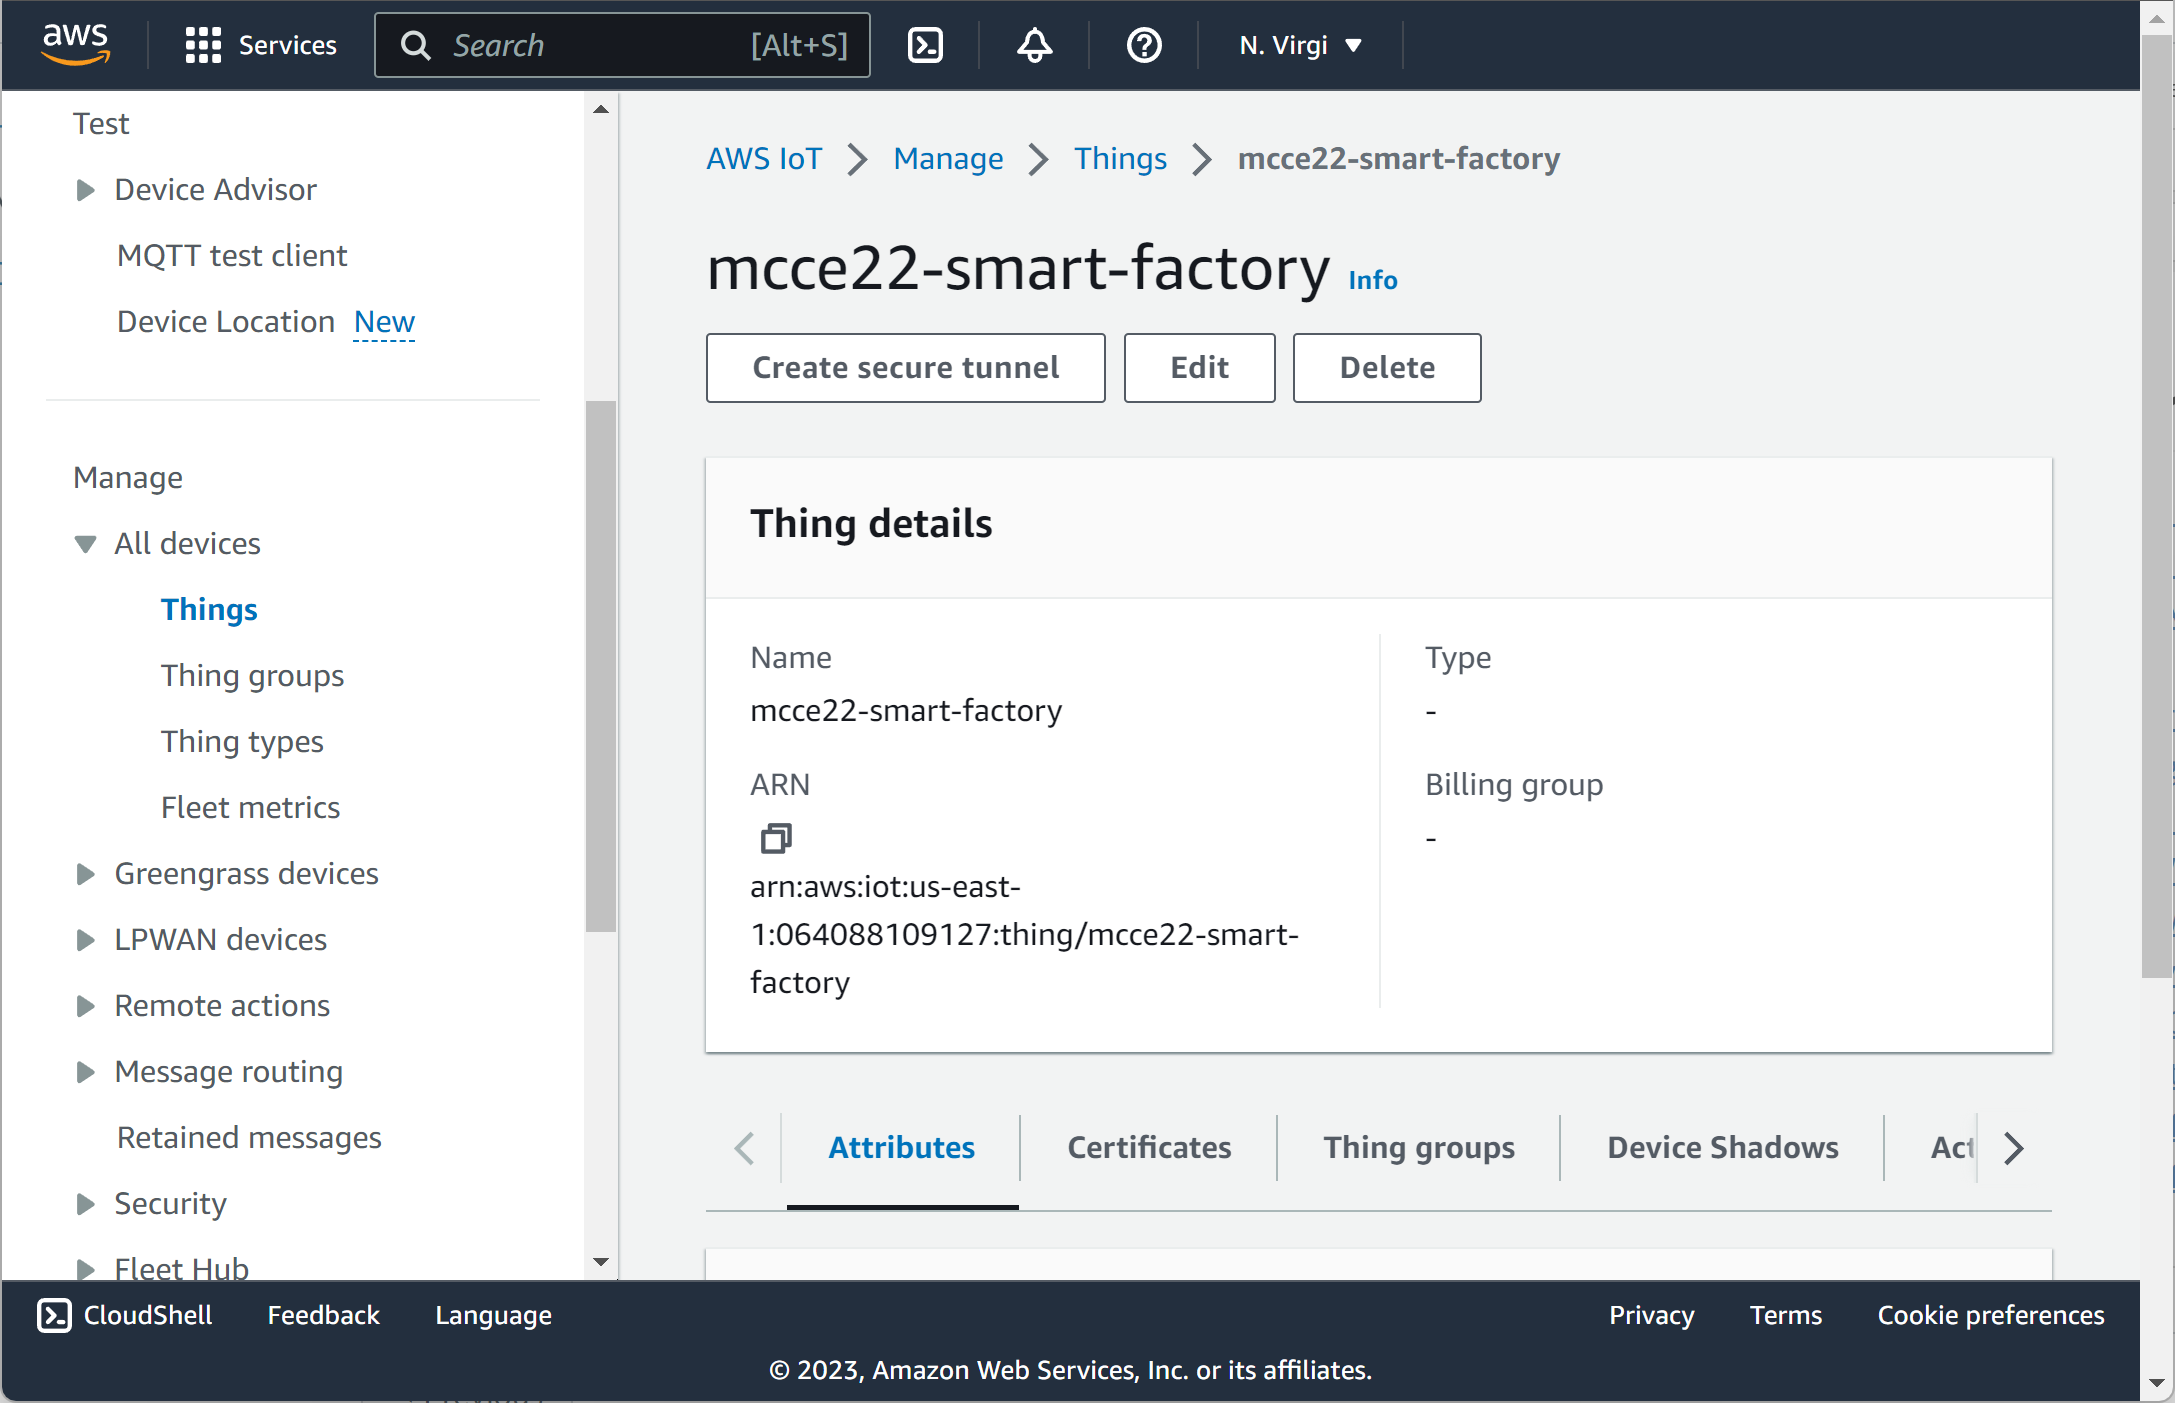
\includegraphics[width=15cm]{images/smart_factory_thing.png}
	\caption{\ac{aws} \ac{iot} Core Thing}    
	\label{fig:SmartFactoryThing}
\end{figure}

Figure \ref{fig:SmartFactoryThing} shows the configuration of such a virtual representation of an \ac{iot} device in \ac{aws} \ac{iot} Core. 
This definition of virtual things is an essential part of IoT Core security system, since a combination of private and public certificate pairs is generated for each defined thing.
These certificates are then required for secure communication with the \ac{aws} \ac{iot} Core Message Broker. 
In the case of our Smart Factory Simulator there is only one client that communicates with the message broker of \ac{aws} \ac{iot} Core and therefore only one virtual thing has been created. 
In a real world scenario, in which each sensor, actuator or button of the smart factory is  represented by its own \ac{iot} device, there would be one thing definition for each physical device.

\section{IoT Simulator}
Initially it was planned to simulate the sensors, actuators and buttons as well as the required control loops using the \ac{aws} \ac{iot} Simulator. 
\ac{aws} \ac{iot} Simulator is a collection of different AWS tools that allow users to test and simulate the behavior of \ac{iot} devices and their interactions with the \ac{aws} \ac{iot} platform without requiring any physical hardware. 
The required tools are provided directly in your own AWS account using infrastructure as code.
Unfortunately, some tools and features required by the \ac{aws} \ac{iot} Simulator were not available in the FH Burgenland \ac{aws} LAB environment, which is why an alternative approach for simulating the Smart Factory \ac{iot} devices had to be chosen.

In order to still be able to show the interaction of the individual sensors, actuators and buttons of the Smart Factory, a small simulator was implemented for the visualization and the implementation of the required control loops. 
Figure \ref{fig:SmartFactorySimulator} shows the Smart Factory simulator and highlighted the implemented use cases.

\begin{figure}[H]
	\centering
	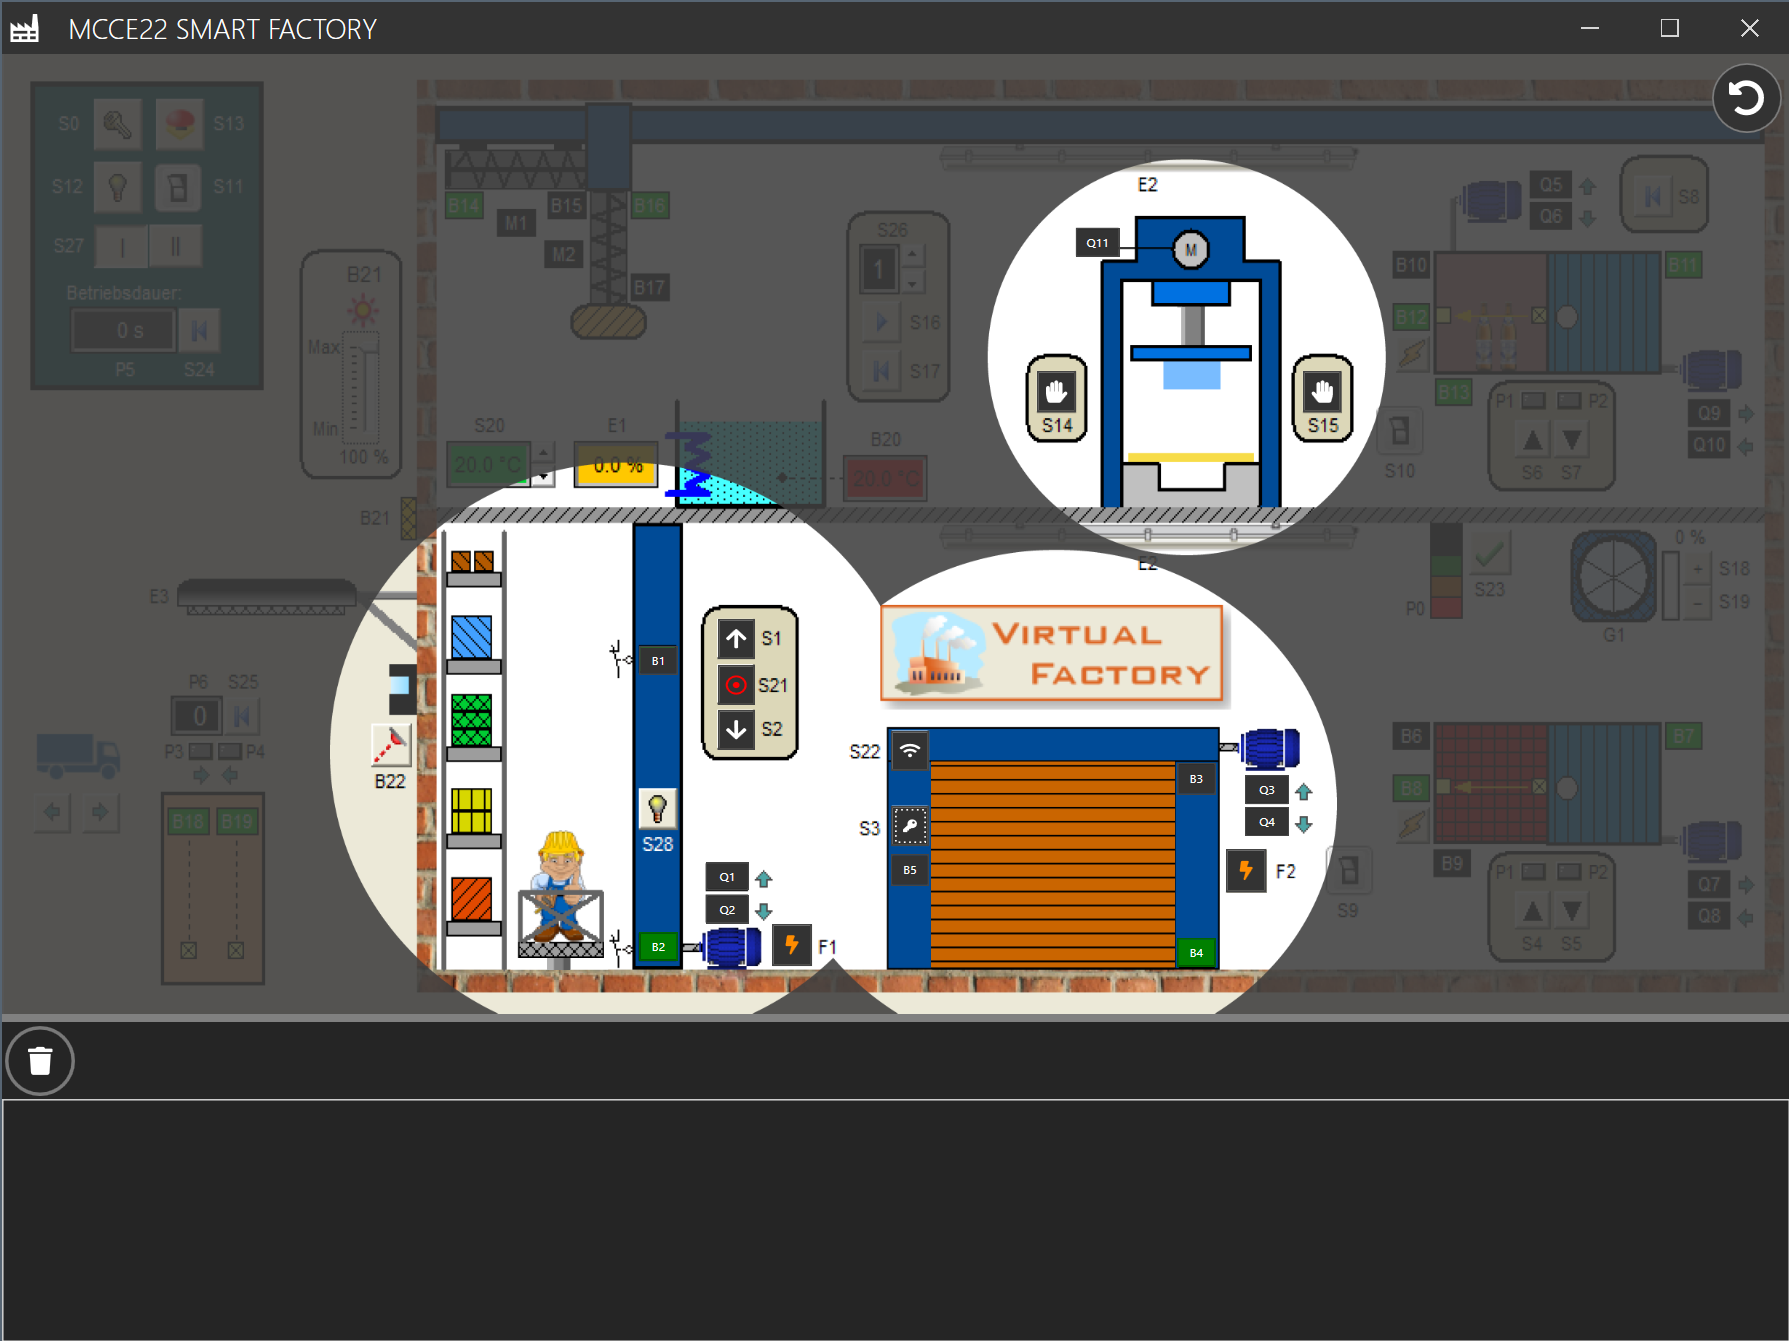
\includegraphics[width=15cm]{images/smart_factory_simulator.png}
	\caption{Smart Factory Simulator}    
	\label{fig:SmartFactorySimulator}
\end{figure}

\textbf{.NET Core}

.NET Core is a free, open-source, cross-platform framework for building modern applications. 
It is a successor to the .NET Framework and provides a set of tools, libraries and runtime environments for building applications for Windows, Linux and macOS operating systems.

\textbf{\ac{wpf}}

\ac{wpf} is a graphics framework of the .NET Framework from Microsoft. 
It provides a powerful set of features for creating visually appealing and interactive user interfaces. \ac{wpf} also includes a rich set of controls that can be used to create common user interface elements such as buttons, text boxes, and menus. 
In addition, WPF offers the possibility to define animations and transitions. 
These animations cabalitites where used to realize the moving transitions of the different parts in the Smart Factory simulator.

\textbf{MaaApps.Metro}

MahApps.Metro is an open-source library that can be used to create modern, stylish and functional Windows desktop applications. 
It's built on Microsoft's \ac{wpf} framework and offers a set of controls, styles, and templates that make it easy to create professional-looking applications.

\textbf{MQTTnet}

MQTTnet is a powerful and open source C\# library to simplify MQTT-based communication. 
In Smart Factory simulator, this library was used to establish the communicate with \ac{aws} \ac{iot} Core.

In order to implement the function of the sensors, actuators and buttons as realistically as possible, a separate class was implemented for each of these components. 
This encapsulation allowed the behavior of each component to be implemented separately and independently. 
All communication between these classes was done exclusively by exchanging MQTT messages using AWS IoT Core. 
Each implementation of a sensor, actuator or button only subscribes to the MQTT topics that is required for its function or control loop. Figure \ref{fig:FlowChartS3} shows the flowchart of the control loops for S3 that were used to automate the factory door. The following \ac{mqtt} topics were defined for the implementation of the 4 use cases:

\begin{itemize}
	\item mcce22-smart-factory/door
	\item mcce22-smart-factory/lifter
	\item mcce22-smart-factory/press
	\item mcce22-smart-factory/light
\end{itemize}

\begin{figure}[H]
	\centering
	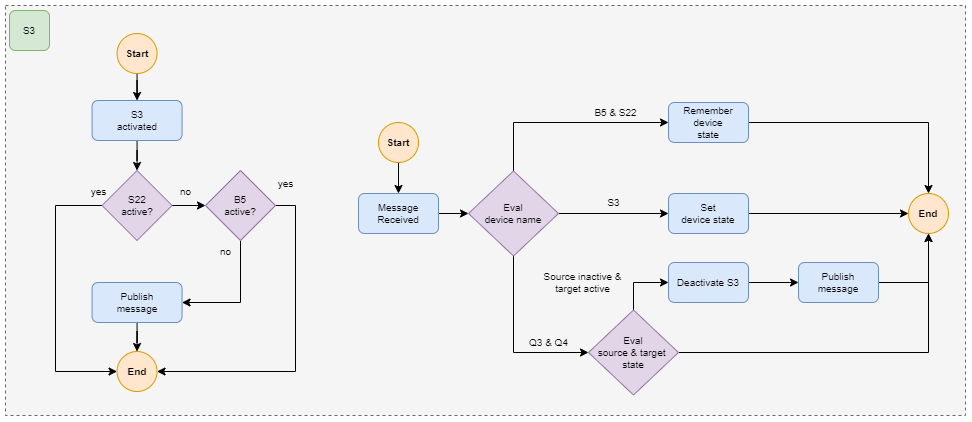
\includegraphics[width=15cm]{images/flowchart_s3.png}
	\caption{S3 Control Loops}    
	\label{fig:FlowChartS3}
\end{figure}

Since S3 is a button, there are two possible control loops. The first describes manually triggering the button while loop two is started by receiving a message from AWS IoT Core. Figure \ref{fig:FlowChartQ3}  shows the control loop for the factory gate motor Q3 and how it is controlled by receiving messages from AWS IoT Core triggered from other sensors or buttons.

\begin{figure}[H]
	\centering
	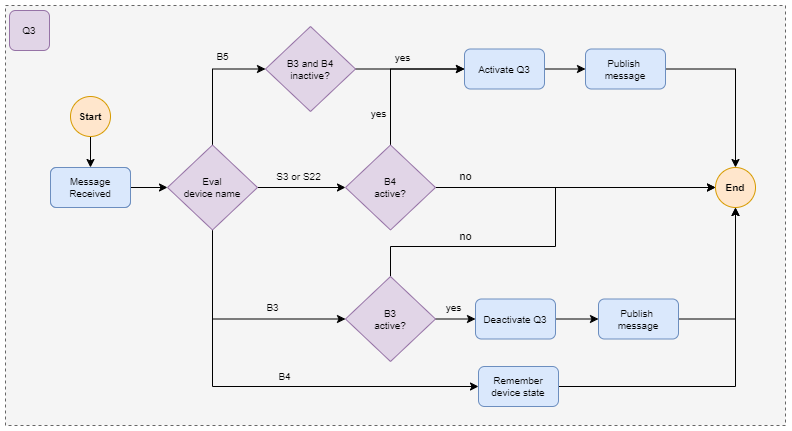
\includegraphics[width=13cm]{images/flowchart_q3.png}
	\caption{Q3 Control Loop}    
	\label{fig:FlowChartQ3}
\end{figure}

\chapter{Use cases}

\section{Assignment}
Setzen Sie den zugewiesenen Use Case um.
Finden Sie dafür ein geeignetes IoT Framework und begründen Sie dessen Eignung für den jeweiligen Case. In unserem Fall \ac{aws}.\\
\\
Inhalt der Seminararbeit (max. 10 Seiten):
\begin{itemize}
    \item Beschreiben Sie das IoT-Framework, Ihr Lösungskonzept und die gewählte technische Umsetzung
    \item Gehen Sie dabei auf Herausforderungen aus technischer und konzeptioneller Sicht sowie auf Security ein
\end{itemize}
Abgabe: 31.5.2023 via Moodle (Seminararbeit + Präsentation). Präsentation: 2.6.2023 – Demonstration des Use Cases erwünscht!

%Zitat \autocite[S. 20]{diekmann2010}



\chapter{Challenges}

\section{Assignment}
Setzen Sie den zugewiesenen Use Case um.
Finden Sie dafür ein geeignetes IoT Framework und begründen Sie dessen Eignung für den jeweiligen Case. In unserem Fall \ac{aws}.\\
\\
Inhalt der Seminararbeit (max. 10 Seiten):
\begin{itemize}
    \item Beschreiben Sie das IoT-Framework, Ihr Lösungskonzept und die gewählte technische Umsetzung
    \item Gehen Sie dabei auf Herausforderungen aus technischer und konzeptioneller Sicht sowie auf Security ein
\end{itemize}
Abgabe: 31.5.2023 via Moodle (Seminararbeit + Präsentation). Präsentation: 2.6.2023 – Demonstration des Use Cases erwünscht!

%Zitat \autocite[S. 20]{diekmann2010}



%	\begin{comment}

%\chapter{Verzeichnisse}
\cleardoublepage
%\appendix
%	\end{comment}
%\chapter{Verzeichnisse}
%http://stackoverflow.com/questions/1243342/how-to-avoid-a-page-break-before-start-of-bibliography
%\nocite{*}
\nocite{back2012web}
\begingroup
\let\clearpage\relax
\printbibliography[heading=bibnumbered] 
\endgroup

\newpage

%\bibliography{References}
\begingroup
\let\clearpage\relax
\listoffigures
\endgroup
\newpage

\begingroup
\let\clearpage\relax
\listoftables
\endgroup
\newpage
\chapter*{Formelverzeichnis}

Nur bei vielen Formeln und Abkürzungen erforderlich bzw. wenn von Betreuungsperson gewünscht.

\begingroup
\let\clearpage\relax
\vspace{-2.5cm}
\listofmyequations
\endgroup
\newpage


\chapter*{Abkürzungen}

\begin{acronym}
    \acro{aws}[AWS]{Amazon Web Services}
    \acro{cd}[CD]{Continuous Delivery/Continuous Deployment}
    \acro{ci}[CI]{Continuous Integration}
    \acro{iac}[IaC]{Infrastructure as Code}
    \acro{sca}[SCA]{Software Composition Analyse}
    \acro{sdlc}[SDLC]{Secure Development Lifecycle}
    \acro{saas}[SaaS]{Software as a Service}
    \acro{sast}[SAST]{Static Application Security Testing}        
\end{acronym}

\newpage
\addcontentsline{toc}{chapter}{Appendix}
\chapter*{Appendix}

\section{Flowcharts}

\subsection*{Factory Gate}

\begin{figure}[H]
    \centering
    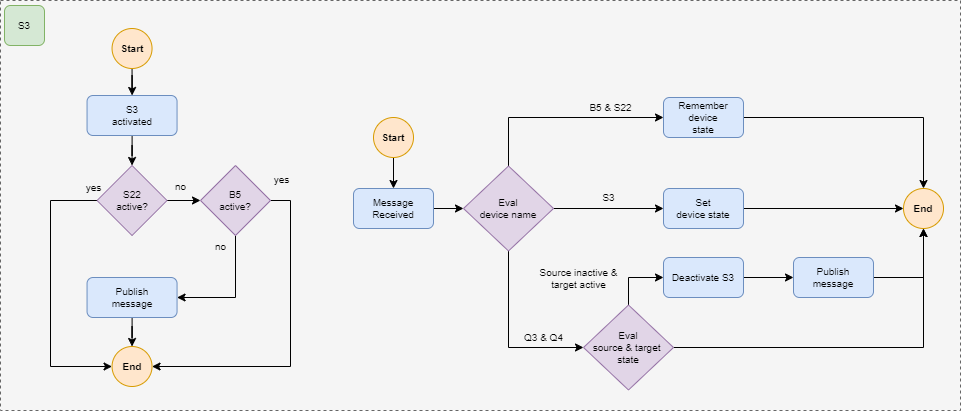
\includegraphics[width=0.9\textwidth]{images/flowchart_factory_gate_s3.png}
    \caption{Flowchart Factory Gate S3}
    \label{fig:FlowChartFactoryDoorS3}
\end{figure}

\begin{figure}[H]
    \centering
    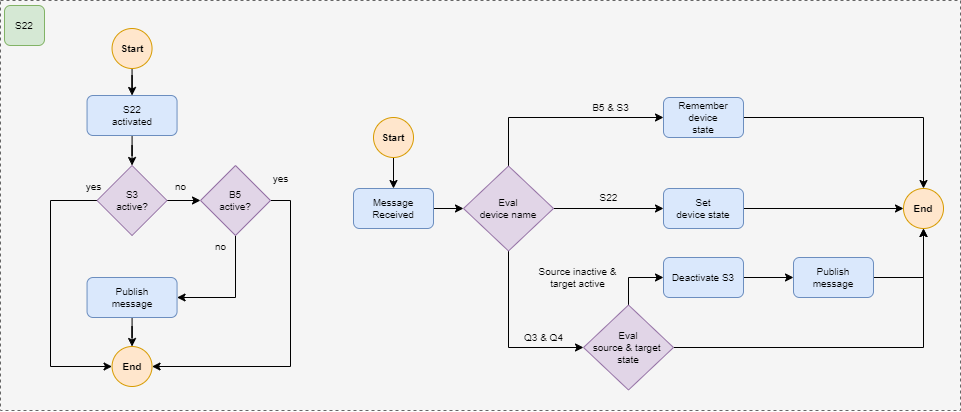
\includegraphics[width=0.9\textwidth]{images/flowchart_factory_gate_s22.png}
    \caption{Flowchart Factory Gate S22}
    \label{fig:FlowChartFactoryDoorS22}
\end{figure}

\begin{figure}[H]
    \centering
    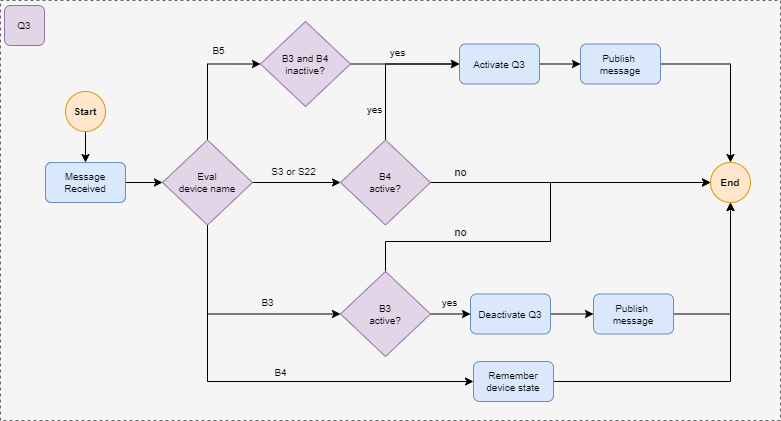
\includegraphics[width=0.9\textwidth]{images/flowchart_factory_gate_q3.png}
    \caption{Flowchart Factory Gate Q3}
    \label{fig:FlowChartFactoryDoorQ3}
\end{figure}

\begin{figure}[H]
    \centering
    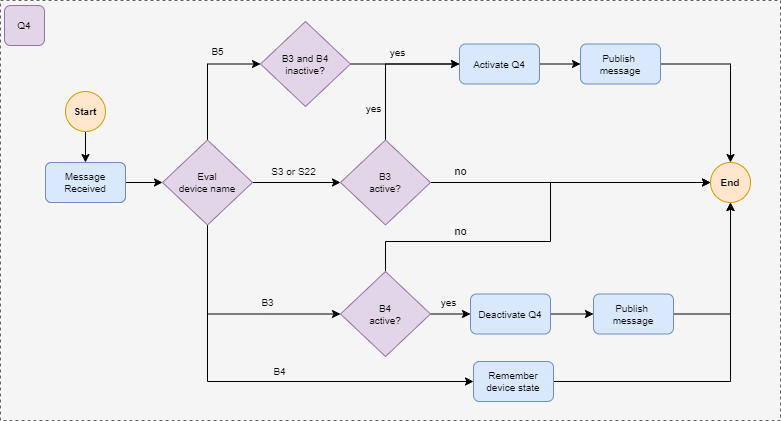
\includegraphics[width=0.9\textwidth]{images/flowchart_factory_gate_q4.png}
    \caption{Flowchart Factory Gate Q4}
    \label{fig:FlowChartFactoryDoorQ4}
\end{figure}

\begin{figure}[H]
    \centering
    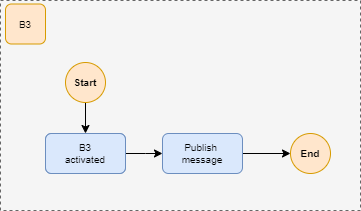
\includegraphics[width=0.5\textwidth]{images/flowchart_factory_gate_b3.png}
    \caption{Flowchart Factory Gate B3}
    \label{fig:FlowChartFactoryDoorB3}
\end{figure}

\begin{figure}[H]
    \centering
    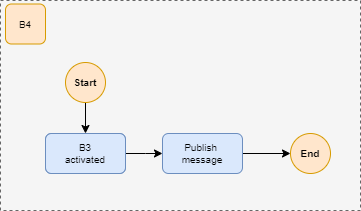
\includegraphics[width=0.5\textwidth]{images/flowchart_factory_gate_b4.png}
    \caption{Flowchart Factory Gate B4}
    \label{fig:FlowChartFactoryDoorB4}
\end{figure}

\begin{figure}[H]
    \centering
    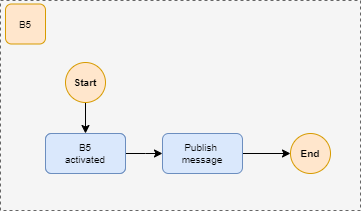
\includegraphics[width=0.5\textwidth]{images/flowchart_factory_gate_b5.png}
    \caption{Flowchart Factory Gate B5}
    \label{fig:FlowChartFactoryDoorB5}
\end{figure}

\subsection*{Lifting Platform}

\begin{figure}[H]
    \centering
    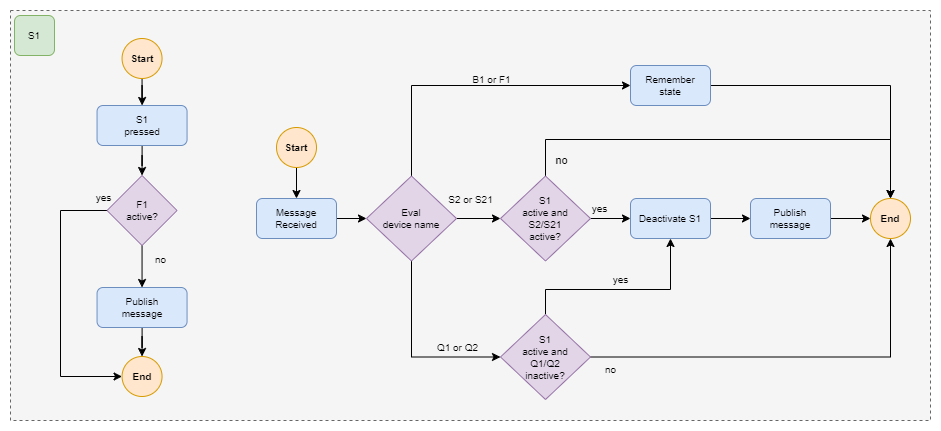
\includegraphics[width=1.0\textwidth]{images/flowchart_factory_lifter_s1.png}
    \caption{Flowchart Factory Lifting Platform S1}
    \label{fig:FlowChartFactoryLifterS1}
\end{figure}

\begin{figure}[H]
    \centering
    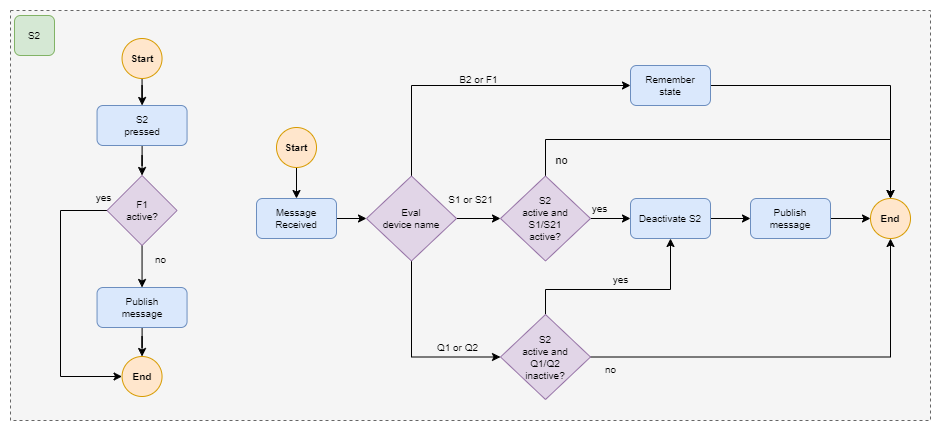
\includegraphics[width=1.0\textwidth]{images/flowchart_factory_lifter_s2.png}
    \caption{Flowchart Factory Lifting Platform S2}
    \label{fig:FlowChartFactoryLifterS2}
\end{figure}

\begin{figure}[H]
    \centering
    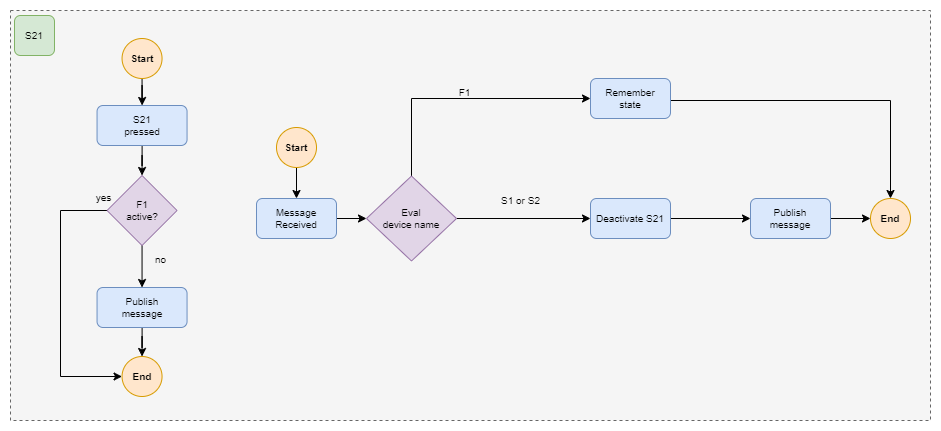
\includegraphics[width=1.0\textwidth]{images/flowchart_factory_lifter_s21.png}
    \caption{Flowchart Factory Lifting Platform S21}
    \label{fig:FlowChartFactoryLifterS21}
\end{figure}

\begin{figure}[H]
    \centering
    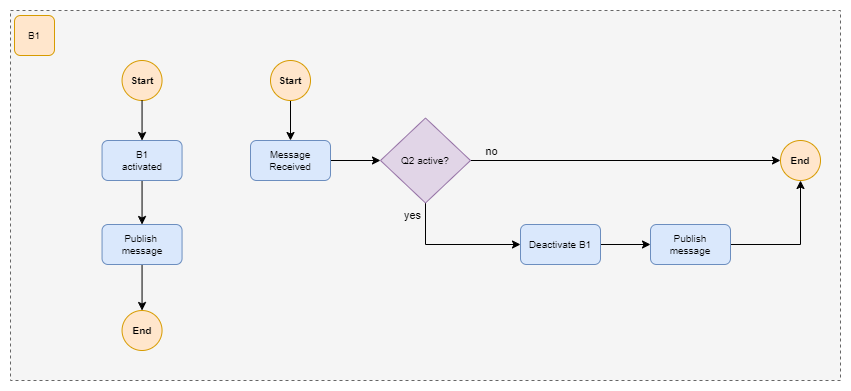
\includegraphics[width=1.0\textwidth]{images/flowchart_factory_lifter_b1.png}
    \caption{Flowchart Factory Lifting Platform B1}
    \label{fig:FlowChartFactoryLifterB1}
\end{figure}

\begin{figure}[H]
    \centering
    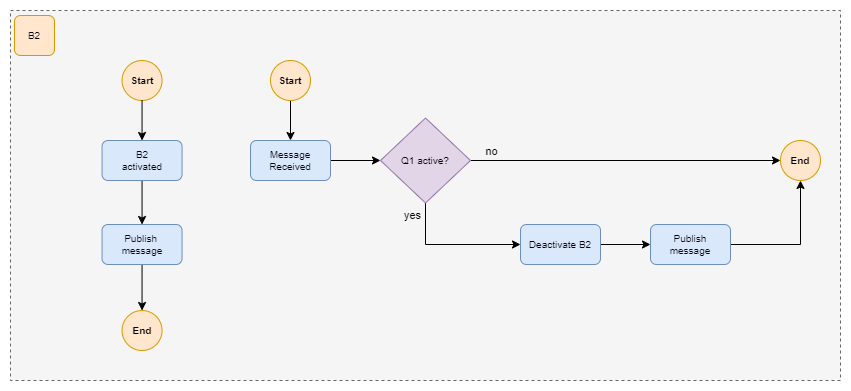
\includegraphics[width=1.0\textwidth]{images/flowchart_factory_lifter_b2.png}
    \caption{Flowchart Factory Lifting Platform B2}
    \label{fig:FlowChartFactoryLifterB2}
\end{figure}

\begin{figure}[H]
    \centering
    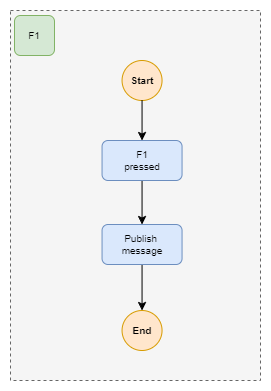
\includegraphics[width=0.4\textwidth]{images/flowchart_factory_lifter_f1.png}
    \caption{Flowchart Factory Lifting Platform F1}
    \label{fig:FlowChartFactoryLifterF1}
\end{figure}

\begin{figure}[H]
    \centering
    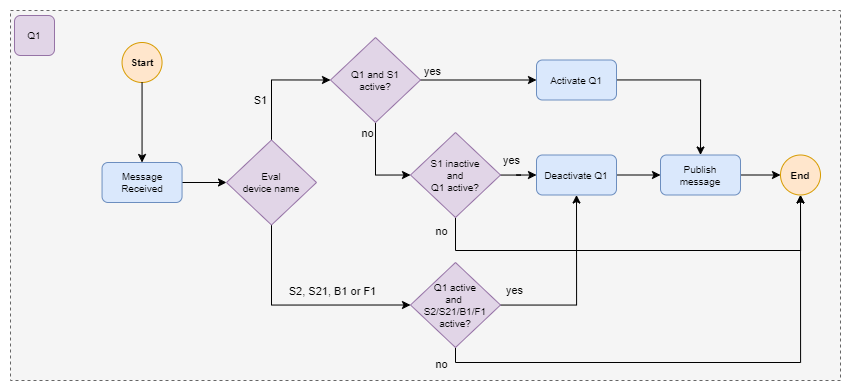
\includegraphics[width=1.0\textwidth]{images/flowchart_factory_lifter_q1.png}
    \caption{Flowchart Factory Lifting Platform Q1}
    \label{fig:FlowChartFactoryLifterQ1}
\end{figure}

\begin{figure}[H]
    \centering
    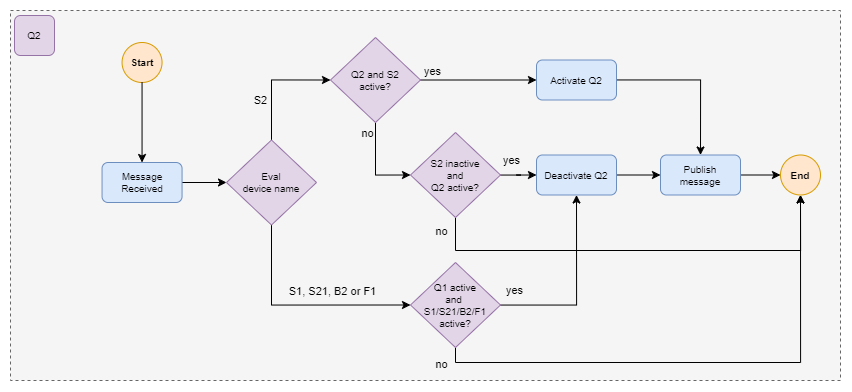
\includegraphics[width=1.0\textwidth]{images/flowchart_factory_lifter_q2.png}
    \caption{Flowchart Factory Lifting Platform Q2}
    \label{fig:FlowChartFactoryLifterQ2}
\end{figure}

\subsection*{Hydraulic Press}

\begin{figure}[H]
    \centering
    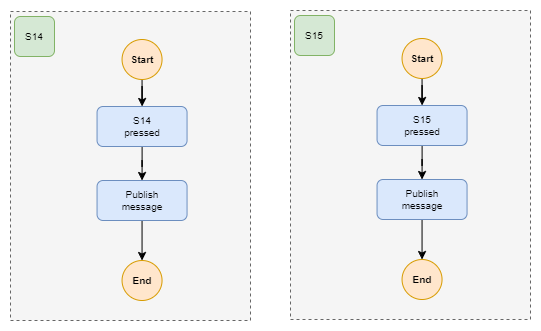
\includegraphics[width=0.7\textwidth]{images/flowchart_factory_press_s14_s15.png}
    \caption{Flowchart Hydraulic Press S14 and S15}
    \label{fig:FlowChartFactoryPressS14S15}
\end{figure}

\begin{figure}[H]
    \centering
    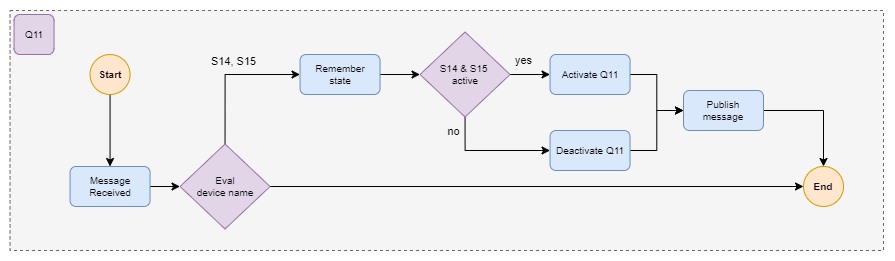
\includegraphics[width=1.0\textwidth]{images/flowchart_factory_press_q11.png}
    \caption{Flowchart Hydraulic Press Q11}
    \label{fig:FlowChartFactoryPressQ11}
\end{figure}

\subsection*{Factory Light}

\begin{figure}[H]
    \centering
    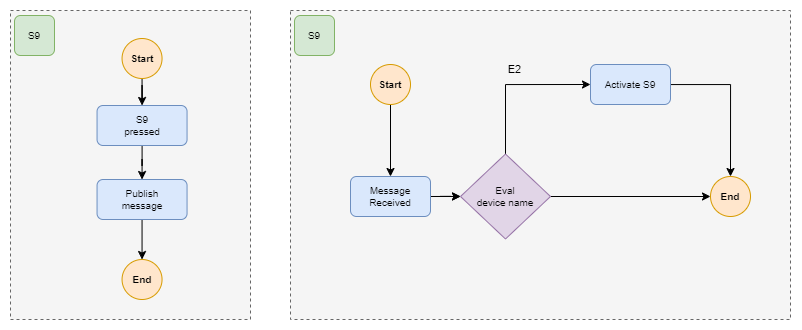
\includegraphics[width=1.0\textwidth]{images/flowchart_factory_light_s9.png}
    \caption{Flowchart Factory Light S9}
    \label{fig:FlowChartFactoryLightS9}
\end{figure}

\begin{figure}[H]
    \centering
    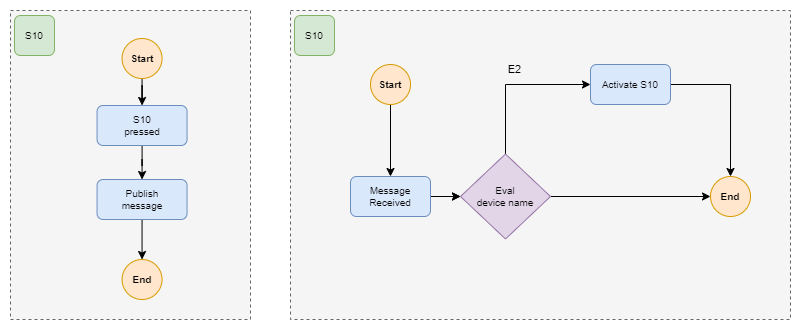
\includegraphics[width=1.0\textwidth]{images/flowchart_factory_light_s10.png}
    \caption{Flowchart Factory Light S10}
    \label{fig:FlowChartFactoryLightS10}
\end{figure}

\begin{figure}[H]
    \centering
    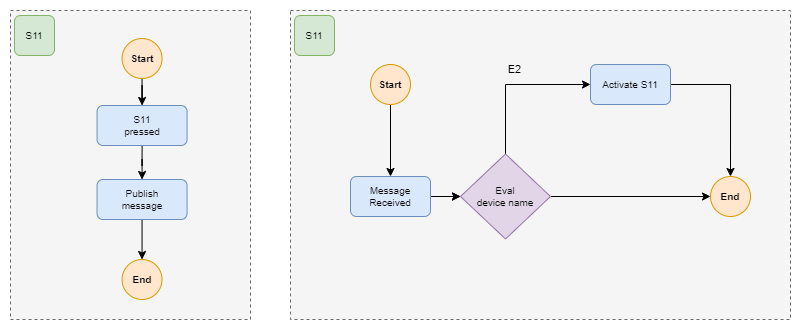
\includegraphics[width=1.0\textwidth]{images/flowchart_factory_light_s11.png}
    \caption{Flowchart Factory Light S11}
    \label{fig:FlowChartFactoryLightS11}
\end{figure}

\begin{figure}[H]
    \centering
    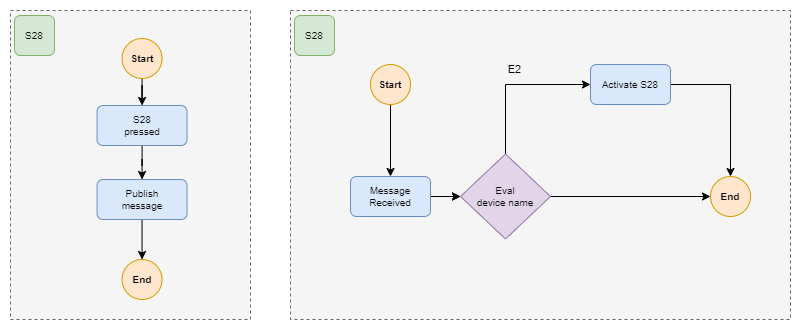
\includegraphics[width=1.0\textwidth]{images/flowchart_factory_light_s28.png}
    \caption{Flowchart Factory Light S28}
    \label{fig:FlowChartFactoryLightS28}
\end{figure}

\begin{figure}[H]
    \centering
    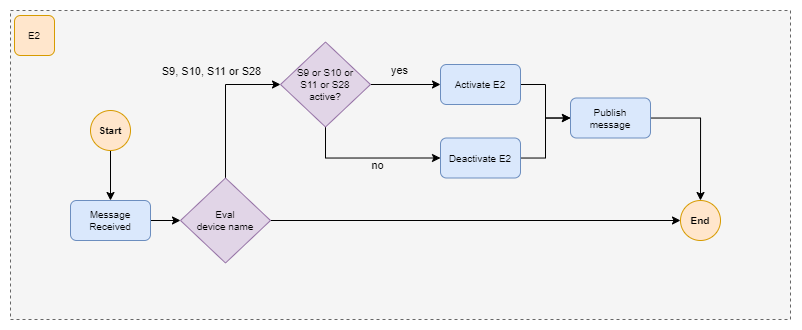
\includegraphics[width=1.0\textwidth]{images/flowchart_factory_light_e2.png}
    \caption{Flowchart Factory Light E2}
    \label{fig:FlowChartFactoryLightE2}
\end{figure}


\end{document}
